\documentclass[11pt,a4paper]{article}

\usepackage[margin=2.3cm]{geometry}
\usepackage[utf8]{inputenc}
\usepackage[T1]{fontenc}
\usepackage{times}
\usepackage{amsmath}
\usepackage{graphicx}
\usepackage{booktabs}
\usepackage{caption}
\usepackage[hidelinks]{hyperref}
\usepackage{enumitem}
\usepackage{titlesec}

\setlength{\parskip}{0.35em}
\setlength{\parindent}{0pt}
\titlespacing*{\section}{0pt}{1.4em}{0.6em}
\titlespacing*{\subsection}{0pt}{1.1em}{0.4em}

\newcommand{\refitem}[1]{\par\noindent\hangindent=1.4em\hangafter=1 #1\par}

\title{\textbf{FarmSense: A Confidence-Aware Crop Digital Twin with Farmer-in-the-Loop Correction for Smallholder Rice Cultivation in Eastern Uttar Pradesh}}

\author{Baiju Yadav \quad Sachin Kumar \quad Ranveer Yadav \quad Anshu Raj\\[2pt]
\small CBS1901 Technical Answers for Real World Problems (TARP)}
\date{}

\begin{document}
\maketitle
\vspace{-1.2em}

\begin{abstract}
\noindent Smallholder rice farmers in the Gangetic plain lack per-field advisory that respects local land units, the ponded water regime of transplanted paddy, and the limits of what an image classifier can safely say. We present FarmSense, a web and mobile advisory system organised around one crop digital twin: a daily simulation of phenology (growing-degree days) and a ponded-depth water balance for bunded paddy, driven by open weather and soil data and corrected by Sentinel-1 radar observations, farmer check-ins and dated leaf photographs. A recommendation engine and a tool-grounded language-model assistant both read the same fused state. Leaf-disease diagnosis uses a ten-class EfficientNet-B0 classifier with a Grad-CAM++ heatmap of where it looked, gated by softmax confidence. We evaluate the system critically and report negative results alongside positive ones. The physical core reproduces the FAO-56 Uccle worked example (3.88 against the published 3.9\,mm/day) and tracks Open-Meteo's independent ET\textsubscript{0} product over a full kharif season at three Gorakhpur points ($r=0.92$--$0.93$, RMSE 0.42--0.44\,mm/day). The paddy water balance closes to rounding error over $10^5$ random days. A simulation study shows farmer check-ins raise agreement on the field's flooded/dry state from 78.8\% with no information to 90--97\% depending on logging and answer quality, but do \emph{not} reduce continuous ponded-depth error, because the check-in question only distinguishes three discrete water levels against a continuous truth. On a held-out validation split drawn from the training sources, the disease classifier reaches 92.8\% accuracy (macro F1 0.940); on a photographically distinct, fully external dataset held out of training entirely, accuracy collapses to 20.1\% (macro F1 0.162), and the confidence gate -- which filters effectively in-distribution -- provides almost no protection under this shift, because the model is badly miscalibrated off-distribution (expected calibration error 0.51 against 0.07 in-distribution). The same gate rejects out-of-distribution, non-leaf inputs far better than an earlier four-class model did (18\% accepted at the deployed 0.65 threshold, against 91\% previously), a substantial but incomplete improvement. The twin architecture and its correction loop are sound; the disease-diagnosis component generalises across photographic domains far worse than its own validation split suggests, and this gap -- not the softmax gate alone -- is the finding that should govern how confidently its output is presented to a farmer.

\vspace{0.4em}
\noindent\textbf{Keywords:} rice crop digital twin; ponded-paddy water balance; Sentinel-1; observation correction; EfficientNet; Grad-CAM++; confidence calibration; LLM tool grounding; smallholder agriculture
\end{abstract}

\section{Introduction}

Most farm holdings in eastern Uttar Pradesh are small, and kharif rice is grown ponded behind bunds, so the question that matters day to day is not how depleted the soil is but how much standing water remains. Over-irrigation wastes pumping fuel and promotes disease, while a dry spell at flowering reduces yield irreversibly through spikelet sterility that cannot be recovered later in the season (Allen et al., 1998; Bouman, Lampayan and Tuong, 2007). Extension advice reaches only a fraction of holdings, and popular smartphone tools are largely diagnostic: they classify a photograph but do not simulate the field, and they quote areas in hectares although farmers think in bigha, katha and dhur.

Three requirements follow. Advice must be per field and per day, because weather, soil and management differ from plot to plot. The system must be honest about uncertainty and must not present a low-confidence or out-of-scope diagnosis as an instruction. It must also work without instruments, since the only sensors a smallholder reliably has are their eyes and a phone camera.

This paper describes FarmSense, a system built around these requirements for rice cultivation, and evaluates it critically. Its contributions are:

\begin{itemize}[leftmargin=1.4em]
\item A crop digital twin coupling a growing-degree-day phenology model with a ponded-depth water balance purpose-built for bunded, puddled lowland rice -- not a relabelled soil-depletion model, which is the wrong state variable for a field whose soil sits at or above saturation all season (Section 3.3).
\item A predict--observe--correct loop with three observation channels: Sentinel-1 SAR, converted into a flooding/transplant signature that is cloud-independent through the monsoon; structured farmer check-ins converted into a corrected ponded-depth estimate; and dated leaf photographs that lower the health estimate only when they disagree with the simulation by more than a noise threshold (Section 3.4).
\item A ten-class EfficientNet-B0 leaf-disease classifier with a Grad-CAM++ explanation overlay, evaluated not only on a conventional validation split but on a fully external, held-out dataset -- the evaluation design that exposes how much of its accuracy is disease-general and how much is dataset-specific shortcut learning (Section 3.3.1, Section 4.8).
\item A tool-grounded assistant that may state agronomic quantities only if the twin returned them, and that forwards the farmer's own credentials so database row-level security applies to the agent exactly as it does to the farmer (Section 3.6).
\item An empirical evaluation that includes negative results: numerical validation against FAO-56, an ET\textsubscript{0} intercomparison over a full season, a water-balance closure test, a simulation study of when check-ins help and hurt, a real Sentinel-1 retrieval experiment, a cross-dataset generalisation test for the classifier, and a confidence-gate stress test against non-leaf inputs (Section 4).
\end{itemize}

No field trial has been run. Section 5 states these limits plainly, and the cross-dataset classifier result in Section 4.8 is, by itself, a reason the photo-diagnosis pathway should not yet be trusted beyond decision support.

\section{Related Work}

\subsection{Image-based plant disease detection}

Convolutional networks trained on leaf photographs reach high accuracy on curated benchmarks (Mohanty, Hughes and Salathé, 2016; Ferentinos, 2018), and mobile deployments have been demonstrated for specific crops (Ramcharan et al., 2019); Kamilaris and Prenafeta-Boldú (2018) survey the wider use of deep learning in agriculture. A recurring caveat is that accuracy on laboratory-style images with uniform backgrounds does not transfer to field photographs. Our classifier is an EfficientNet-B0 (Tan and Le, 2019) fine-tuned on ten rice leaf-disease classes merged and cross-deduplicated from several public rice-leaf datasets, replacing an earlier four-class ResNet-18 (He et al., 2016) baseline that we retain in Section 4.8 purely as a comparison point. Section 4.8 shows why accuracy on a single dataset's own validation split, the number most such papers report, is not a safe estimate of field performance.

\subsection{Crop models and digital twins}

Process-based crop models such as DSSAT (Jones et al., 2003), APSIM (Keating et al., 2003) and AquaCrop (Raes et al., 2009) simulate growth and water use but need cultivar, soil and management inputs that smallholders cannot supply, and they are seldom coupled to live observations. The FAO-56 method (Allen et al., 1998) is far lighter: Penman--Monteith reference evapotranspiration is scaled by a crop coefficient. For ponded rice specifically, FAO-56 itself treats paddy as a special case whose state is the depth of standing water rather than a soil-moisture depletion fraction, and IRRI's water-management guidance (Bouman, Lampayan and Tuong, 2007) is written around that same variable. The digital-twin concept (Grieves and Vickers, 2017) has been adopted in smart-farming reviews (Verdouw et al., 2021; Wolfert et al., 2017), which stress the closed loop between the physical asset and its virtual counterpart. Data assimilation methods such as the ensemble Kalman filter (Evensen, 2003) formalise that loop but need an error model for the simulator. We use a confidence-weighted blend that needs none (Section 3.4).

\subsection{Satellite grounding for rice}

Monsoon cloud makes optical satellite data unreliable for kharif rice for weeks at a time. Sentinel-1 C-band radar (Torres et al., 2012) is cloud-independent, and the drop in VH backscatter when a paddy is flooded, followed by recovery as the canopy grows, underlies several rice-mapping methods (e.g.\ Bazzi et al., 2019). We use this signature as an independent, physical check on the farmer-reported transplant date, through the free Copernicus Data Space Ecosystem.

\subsection{Grounded language-model assistants}

Language models can produce fluent but unsupported statements (Ji et al., 2023). Retrieval and tool use mitigate this by conditioning the answer on external evidence (Lewis et al., 2020; Yao et al., 2023). In agronomy the risk is concrete, since a hallucinated dose is an instruction to spray. We therefore constrain the assistant so that agronomic quantities can originate only from tool calls into the twin.

\subsection{Confidence, calibration and out-of-distribution inputs}

Modern networks are often over-confident (Guo et al., 2017), and the maximum softmax probability is only a baseline for detecting inputs the model was not trained on (Hendrycks and Gimpel, 2017). A closed-set classifier has no ``none of the above'' output, yet many agricultural apps present the top class with a confidence percentage. Section 4.8 quantifies the consequence for our system under two distinct failure modes -- non-leaf inputs, and leaf photographs from a camera and background the model has never seen -- and shows that a single softmax gate behaves very differently against each.

\section{System Design}

\subsection{Architecture}

FarmSense has three tiers (Figure~\ref{fig:arch}). React web and Expo (React Native) mobile clients handle field and crop management, photo capture and chat, and talk only to the Node.js/Express backend over the farmer's own bearer token. The backend owns the twin: it ingests weather, soil and Sentinel-1 data, runs the simulation, applies the confidence gate, and serves recommendations. A Python/FastAPI service, reachable only with a shared service token, hosts the image classifier and the LangGraph chat agent; it is never reached directly by a client. Postgres (Supabase) stores fields, crops, daily crop states, check-ins and image records, with row-level security (RLS) so tenant isolation is enforced by the database rather than by application filters. Figure~\ref{fig:dataflow} traces the request path for a single leaf-photo diagnosis end to end, since this is the path where the architecture's safety properties -- the service token boundary, the confidence gate, and the twin correction step -- all have to compose correctly.

\begin{figure}[htbp]
\centering
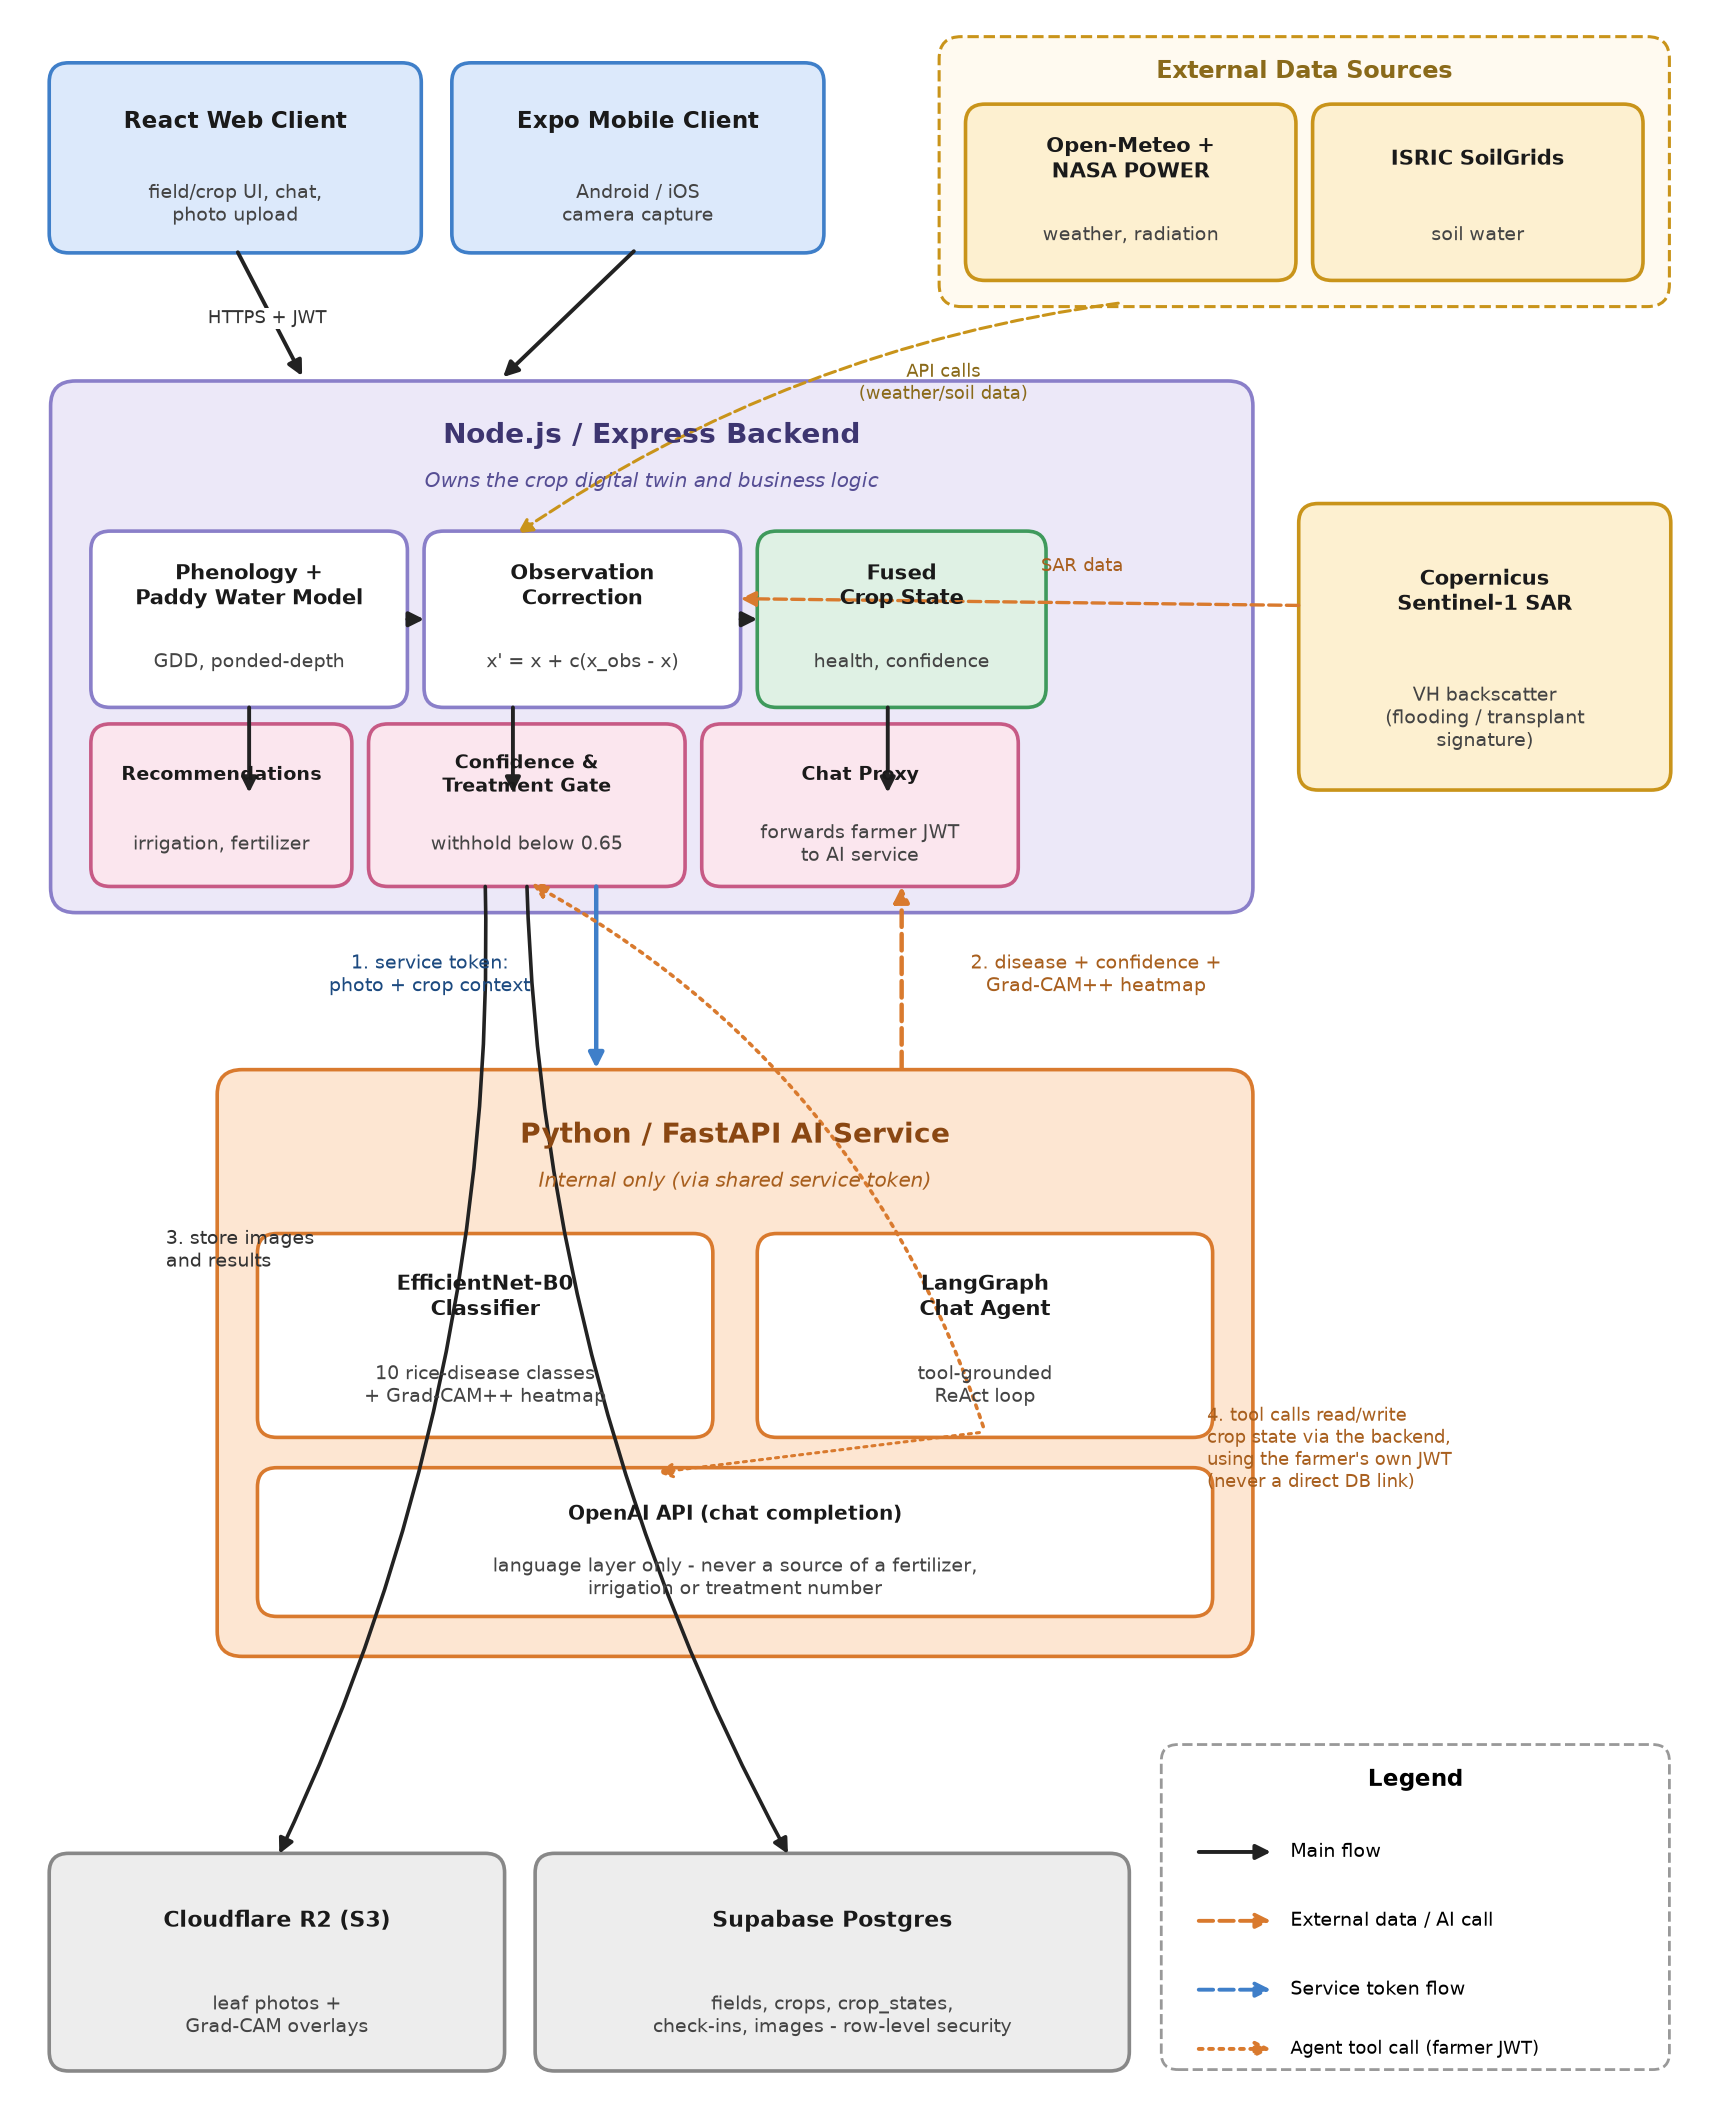
\includegraphics[width=0.92\textwidth]{fig/arch.png}
\caption{FarmSense system architecture, with the disease-diagnosis request numbered end to end. Clients reach only the Express backend. Open weather and soil data drive the phenology and paddy water models; Sentinel-1 SAR corrects the fused state through the same operator as farmer check-ins and dated photographs. The AI service is internal, reached only with a service token (1); its classification response returns to the backend's own confidence gate, never straight to a client (2); images and results are stored from that same disease pathway (3); and the chat agent's tool calls read and write crop state only by calling back into the backend with the farmer's own credentials, never with a direct database connection (4).}
\label{fig:arch}
\end{figure}

\begin{figure}[htbp]
\centering
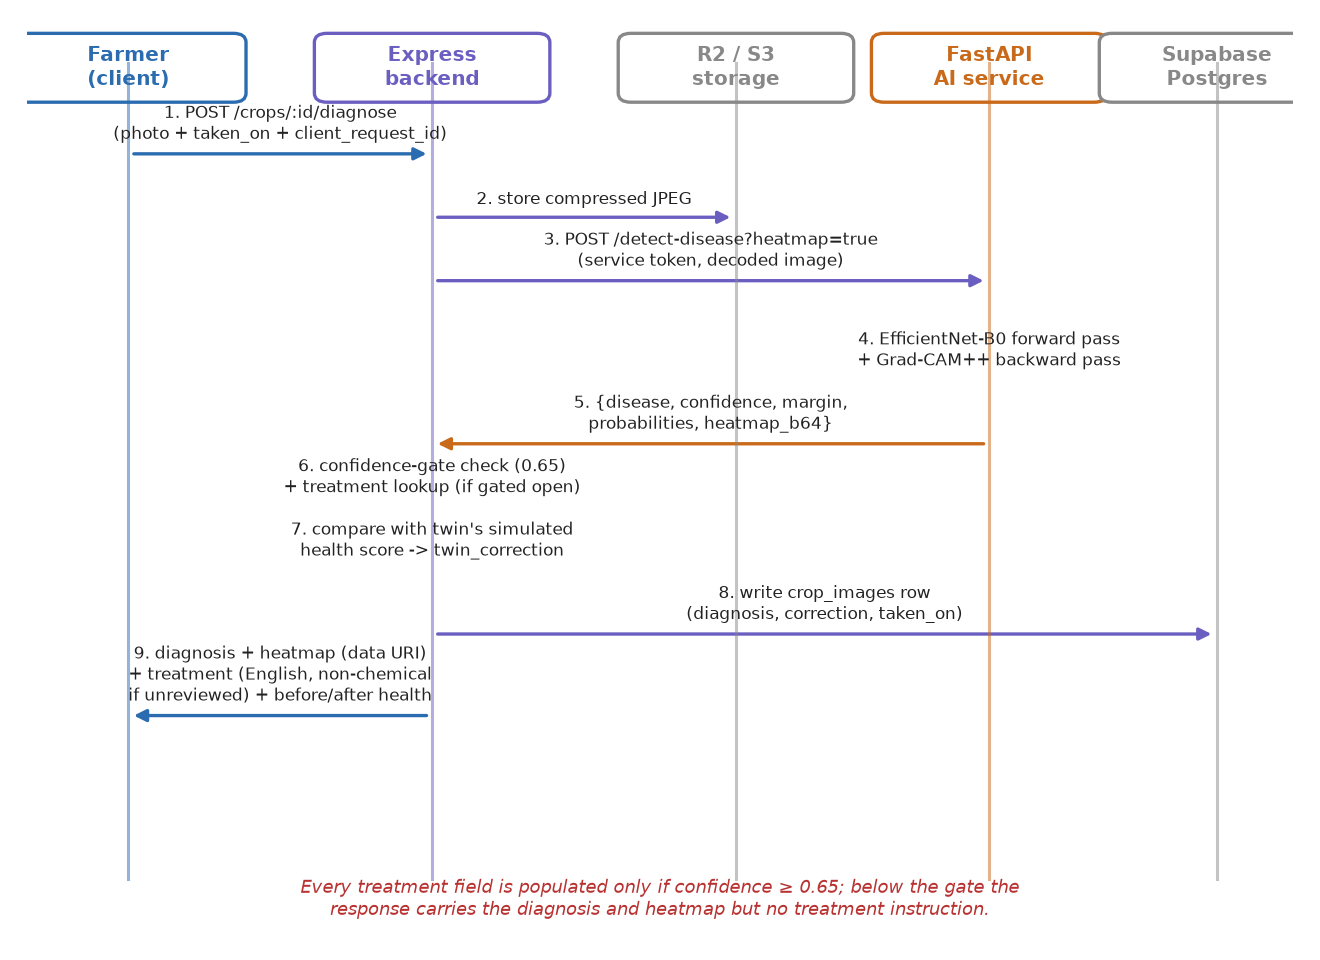
\includegraphics[width=0.92\textwidth]{fig/dataflow.png}
\caption{Data flow for one disease-diagnosis request. The treatment field is populated only when the classifier's confidence clears the 0.65 gate; below it, the farmer still receives the diagnosis, its confidence, and the Grad-CAM++ heatmap, but no instruction.}
\label{fig:dataflow}
\end{figure}

\subsection{Phenology and reference evapotranspiration}

Growth stage is driven by thermal time rather than the calendar. With daily maximum and minimum temperatures $T_{max}$ and $T_{min}$ and crop base temperature $T_b$, cumulative growing-degree days on day $n$ are
\begin{equation}
GDD(n) = \sum_{d=1}^{n} \max\!\big(0,\ (T_{max,d}+T_{min,d})/2 - T_b\big)
\end{equation}
Phase boundaries, the crop coefficient $K_c$ and canopy development are indexed to this quantity, so a single confirmed phenological event re-anchors the rest of the season (Section 3.4). Reference evapotranspiration follows the FAO-56 Penman--Monteith equation (Allen et al., 1998):
\begin{equation}
ET_0 = \frac{0.408\,\Delta\,(R_n - G) + \gamma \dfrac{900}{T+273} u_2 (e_s - e_a)}{\Delta + \gamma (1 + 0.34\,u_2)}
\end{equation}
Net radiation $R_n$ is derived from measured shortwave radiation, $\Delta$ is the slope of the vapour-pressure curve, $\gamma$ the psychrometric constant at the field's elevation, $u_2$ the 2\,m wind speed (floored at 0.5\,m/s) and $e_s-e_a$ the vapour-pressure deficit. Shortwave radiation and wind come from NASA POWER (Sparks, 2018); temperature, humidity and rainfall come from Open-Meteo (Zippenfenig, 2023). When radiation or wind is missing the system falls back to the Hargreaves--Samani equation and lowers its reported confidence; every simulated day in the experiments below used Penman--Monteith.

\subsection{The ponded-depth water model}
\label{sec:paddy}

An earlier internal prototype of this system ran rice through the same soil-depletion bucket used for upland crops -- the wrong model, not a simplification of the right one. A puddled paddy's soil sits at or above saturation essentially all season; ``depletion below field capacity'' is not a meaningful quantity there, losses are dominated by percolation through the compacted plough pan rather than root-zone extraction, and the crop's stress trigger is the water layer disappearing, not a gradual soil-moisture decline. The model reported here instead tracks ponded depth $h$, the water standing above the soil surface, following FAO-56's own treatment of rice as a special case and IRRI water-management guidance (Bouman, Lampayan and Tuong, 2007):
\begin{equation}
h_{n} = \min\!\big(h_{bund},\ \max(0,\ h_{n-1} + P_n + I_n - ET_{c,n} - perc_n)\big)
\end{equation}
Rainfall and irrigation land first; water above the bund height $h_{bund}$ (default 150\,mm) overflows and is lost. While the field is flooded, percolation is charged at a near-constant rate (default 3\,mm/day for puddled clay loam). If the day's losses exceed standing water, the pond empties and the remaining demand draws on a small saturated soil buffer (default 40\,mm) before the field is counted as dry; a dry-day counter starts, and the day resets to zero the moment irrigation or rain above 20\,mm re-floods the field. Dryness during flowering is flagged as critical, since spikelet sterility from a water deficit at that stage cannot be reversed by better management afterwards; dryness during grain-filling and maturity is not a stress signal, since draining before harvest is deliberate practice.

We tested this model for closure and bounds over $10^5$ random days spanning realistic rainfall, irrigation, demand and starting-state ranges (Section 4.2): across all of them it never reported a ponded depth below zero or above the bund height, never reported a soil buffer beyond its own cap, and never removed more water on a single day than the day's standing water plus the full buffer could supply.

\subsection{Observation channels and the correction operator}

Simulations drift: irrigation is left unlogged, soils differ from their SoilGrids estimate, and cultivars mature at their own pace. FarmSense assimilates three observation channels, and all of them share one operator that moves a state variable $x$ toward an observed target $x_{obs}$ in proportion to the observation's confidence $c \in [0,1]$:
\begin{equation}
x' = x + c\,(x_{obs} - x)
\end{equation}
At $c=1$ the observation wins outright, and at $c=0$ the simulation is untouched. This avoids specifying error variances for a simulator whose error is uncharacterised, at the price of a fixed trust weight per observation type -- a limitation examined in Section 4.6.

\textbf{Farmer check-ins.} A short question (``is the field flooded?'') is answered by tapping one of three options -- deep standing water, shallow standing water, or drained -- each mapped to a target ponded depth (50, 15 and 0\,mm respectively) with its own confidence (0.90, 0.85, 0.90). A ``drained'' answer when the simulation still predicts standing water also flags the percolation-rate parameter for recalibration, since that is the input most likely to be wrong, not the day's weather.

\textbf{Satellite.} Sentinel-1 VH backscatter in dB is examined for the flooding signature through the Copernicus Data Space Statistical API: a minimum below $-22$\,dB with at least 3\,dB of descent and 3\,dB of recovery is reported as a transplant event, with a confidence combining the depth and shape of the dip.

\textbf{Dated photographs.} A farmer uploads a leaf photograph and states the date it was taken. If the diagnosis clears the confidence gate, the classifier's health score becomes an upper bound (a ceiling, never a floor) on that day's simulated health, applied only when the simulation exceeds it by more than 10 points -- the same bounded-correction logic as a farmer check-in, with the photo's own confidence fading linearly to zero over the following 7 days, since disease does not vanish overnight but a photo also should not keep correcting the twin indefinitely. A healthy leaf is deliberately not used to raise the estimate, because it says nothing about water stress.

\subsection{Confidence and the treatment gate}

Each state carries a confidence report that falls with staleness of the last observation, use of fallback soil data, absence of a traced field boundary, and time since the last check-in, and that is lowered when an observation disagreed with the simulation. Below a threshold the system advises inspecting the field or contacting the local extension officer. For diagnoses, the classifier's top-class probability is compared with a gate (default 0.65); below it the response carries the diagnosis and the Grad-CAM++ heatmap but no treatment field at all, so a client cannot display advice the service declined to stand behind (Figure~\ref{fig:dataflow}, step 6). Section 4.8 evaluates this gate against two different threats and finds it effective against one and not the other.

\subsection{Tool-grounded assistant}

The chat assistant is a tool-calling agent in the ReAct pattern (Yao et al., 2023), implemented with LangGraph. Its tools return the fused crop state, the irrigation recommendation and the fertilizer plan, and its system prompt forbids stating any fertilizer quantity, irrigation volume, pesticide or dose that did not come from a tool result; it is also instructed to always reply in English regardless of the language the farmer writes in, so that crop and place names stay unambiguous across a mixed Hindi/Bhojpuri/English farmer population. Before answering a crop-specific question, the agent is given a short prefetched summary of the crop and field (crop type, field name, sowing date, status) rather than a bare database identifier, so it can ground an answer without first having to call a tool just to find out what it is being asked about. The tools call the backend with the farmer's own access token rather than a service key, so row-level security applies to the agent exactly as it does to the farmer: the agent cannot read another user's field even if asked.

\subsection{Regional configuration and local units}

All agronomic constants (the $K_c$ curve, growing-degree-day boundaries, paddy bund geometry, fertilizer rates and the land-unit ladder) reside in a region file selected by an environment variable and served to the client, so neither the engine nor the interface contains a district name. The deployed calibration is Gorakhpur district ($26.76^{\circ}$N, $83.37^{\circ}$E). Areas are entered in the customary pucca-bigha ladder (1 bigha = 20 katha = 400 dhur = 2{,}529.3\,m\textsuperscript{2}) and converted once, server-side; fertilizer quantities are returned in kilograms and 50\,kg sacks. Field locations are chosen on a map and validated to lie inside the district, since advice for a point outside the calibrated region would look authoritative and be wrong.

\section{Experimental Evaluation}

\subsection{Scope, data and reproducibility}

No soil-moisture measurements or farmer trials were available. The evaluation uses: (i) published FAO-56 worked examples; (ii) real historical weather and soil data for a full kharif season at three pre-specified points in Gorakhpur district (P1 $26.76^{\circ}$N $83.37^{\circ}$E; P2 $26.40^{\circ}$N $83.10^{\circ}$E; P3 $27.00^{\circ}$N $83.70^{\circ}$E), simulating rice transplanted on 1 July 2025 for 140 days; (iii) real Sentinel-1 retrievals; (iv) a simulation study with an explicit, synthetic farmer-error model; (v) the shipped disease classifier's own training-run metrics, which separate an in-distribution validation split from a fully external held-out dataset; and (vi) a stress test of the shipped classifier against non-leaf inputs, together with a qualitative case study on five real field photographs supplied for this paper and not part of the training or evaluation corpus. Where an experiment is a consistency check rather than validation against ground truth, we say so. Random processes use fixed seeds, and all reported numbers are produced by scripts that read the raw result files.

At P1, the district centre inside the Gorakhpur urban area, SoilGrids returned no water-retention layers on any attempt, so the regional default (150\,mm/m) was used. At P2 and P3 it gave 212.8 and 172.3\,mm/m, so the fallback path was exercised in practice.

\subsection{Numerical validation of the physical core}

Component functions reproduce FAO-56 worked examples: saturation vapour pressure at $24.5^{\circ}$C, 3.075\,kPa (published 3.075); psychrometric constant at 1{,}800\,m, 0.0544\,kPa/$^{\circ}$C (published 0.054); and extraterrestrial radiation at $20^{\circ}$S on day 246, 32.19\,MJ\,m\textsuperscript{-2}\,day\textsuperscript{-1} (published 32.2). For the complete Penman--Monteith chain we used the Uccle (Belgium) 6 July example of Chapter 4 of the FAO paper ($T_{max}$ 21.5$^{\circ}$C, $T_{min}$ 12.3$^{\circ}$C, RH$_{max}$ 84\%, RH$_{min}$ 63\%, $u_2$ 2.078\,m/s, $R_s$ 22.07\,MJ\,m\textsuperscript{-2}\,day\textsuperscript{-1}, 100\,m, 50.8$^{\circ}$N). The code returns $ET_0 = 3.88$\,mm/day against the published 3.9.

We also tested the ponded-depth water balance (Section~\ref{sec:paddy}) for closure and bounds on $10^5$ random days (starting ponded depth 0--150\,mm, starting soil-buffer drying 0--40\,mm, crop demand 0--9\,mm/day, rainfall up to 100\,mm on 30\% of days, irrigation up to 60\,mm on 15\% of days). Across all $10^5$ days the model never produced a ponded depth below zero or above the 150\,mm bund, never produced a soil-buffer value outside $[0,40]$\,mm, and never removed more water on a single day than that day's standing water plus the full buffer could physically supply. The field was reported as overflowing its bund on 13.0\% of sampled days and as newly dry on 3.1\%, confirming both code paths were genuinely exercised rather than trivially unreachable.

\subsection{Intercomparison of ET\textsubscript{0} over a full season}

Open-Meteo publishes its own FAO-56 ET\textsubscript{0}. Because it is a model product rather than a measurement, agreement is an intercomparison, not a validation, but it independently checks our input handling (NASA POWER radiation and wind combined with Open-Meteo temperature and humidity). Over 420 point-days of the rice season, our ET\textsubscript{0} correlated with Open-Meteo's at $r=0.92$--$0.93$, with RMSE 0.42--0.44\,mm/day and a small negative bias ($-0.20$ to $-0.05$\,mm/day; Table~\ref{tab:eto}, Figure~\ref{fig:eto}).

\begin{table}[htbp]
\centering
\caption{Agreement between FarmSense ET\textsubscript{0} and Open-Meteo ET\textsubscript{0} (mm/day) over the full simulated rice season.}
\label{tab:eto}
\begin{tabular}{lccccccc}
\toprule
Point & $n$ (days) & Mean ours & Mean OM & Bias & RMSE & $r$ \\
\midrule
P1 & 140 & 3.61 & 3.80 & $-0.18$ & 0.43 & 0.93 \\
P2 & 140 & 3.59 & 3.79 & $-0.20$ & 0.44 & 0.92 \\
P3 & 140 & 3.61 & 3.66 & $-0.05$ & 0.42 & 0.92 \\
\bottomrule
\end{tabular}
\end{table}

\begin{figure}[htbp]
\centering
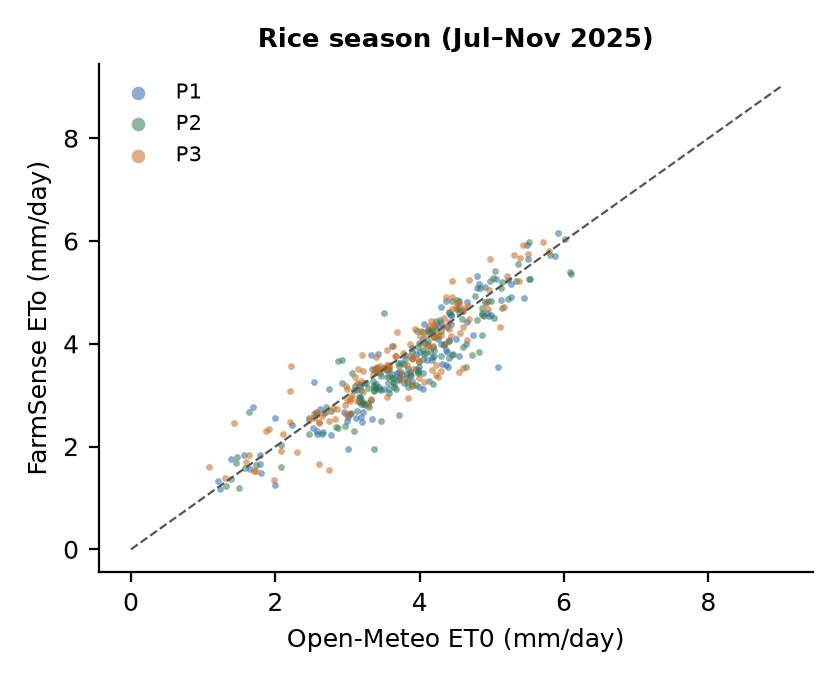
\includegraphics[width=0.55\textwidth]{fig/eto.png}
\caption{Daily FarmSense ET\textsubscript{0} against Open-Meteo ET\textsubscript{0} for the rice season at three Gorakhpur points; the dashed line is 1:1.}
\label{fig:eto}
\end{figure}

\subsection{Season simulation}

Table~\ref{tab:season} summarises the simulated season. Rainfall (757--970\,mm) exceeded crop evapotranspiration (521--526\,mm) at all three points, so the monsoon alone supplies most of the water a paddy needs; the question is whether it arrives evenly enough to keep the field flooded. Without any irrigation the field was unflooded for 25--36 of the 140 days (Figure~\ref{fig:pond}), concentrated early in the season and during dry spells, but \emph{none} of those dry days fell during the flowering phase at any of the three points this season -- the monsoon's timing, not its total, is what protected the critical window here, and that is a property of this particular season's rainfall distribution, not a guarantee.

\begin{table}[htbp]
\centering
\caption{Simulated season totals (mm) from real weather, rice transplanted 1 July 2025. GDD is thermal time accumulated over the 140-day period.}
\label{tab:season}
\begin{tabular}{lccccc}
\toprule
Point & Rain & ET\textsubscript{0} & ET\textsubscript{c} & GDD & Soil source (TAW, mm/m) \\
\midrule
P1 & 757 & 506 & 524 & 2495 & regional default (150.0) \\
P2 & 797 & 503 & 521 & 2480 & SoilGrids (212.8) \\
P3 & 970 & 506 & 526 & 2427 & SoilGrids (172.3) \\
\bottomrule
\end{tabular}
\end{table}

\begin{figure}[htbp]
\centering
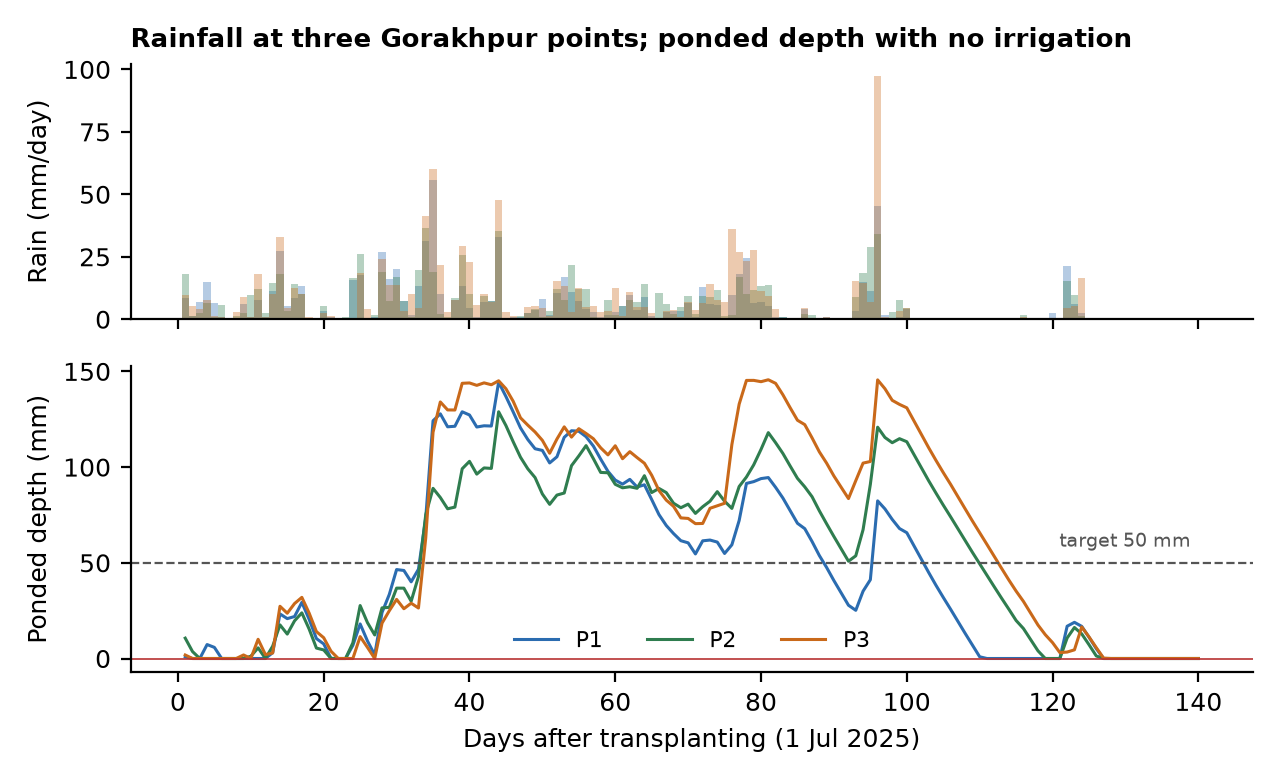
\includegraphics[width=0.72\textwidth]{fig/rice_pond.png}
\caption{Rice season (transplanted 1 July 2025): daily rainfall and simulated ponded depth with no irrigation at three points. Depth is capped by the 150\,mm bund.}
\label{fig:pond}
\end{figure}

\subsection{Ponding-management consistency}

We compared the no-irrigation case above with a simple refill policy -- top up to the 50\,mm target depth whenever the pond falls below 20\,mm -- on the same weather (Table~\ref{tab:ponding}, Figure~\ref{fig:ponding_sat} left). Keeping the field continuously flooded required 5--7 refills totalling 182--245\,mm of net irrigation. Bund overflow, water lost over the bund during heavy rain, was substantial even under the refill policy: negligible at P1 and P2 but 210\,mm at P3, the wettest point (970\,mm of seasonal rain), because the policy as implemented refills to a fixed 50\,mm target without anticipating rainfall already in the forecast. This is a genuine inefficiency: at a point that already receives abundant monsoon rain, a policy that reacts only to the current pond level, rather than to short-range rainfall forecasts, both irrigates and loses more water than necessary over the season. A forecast-aware refill rule is a direct, low-risk improvement the twin's architecture already has the inputs for.

\begin{table}[htbp]
\centering
\caption{Ponding-management consistency: no irrigation vs.\ a reactive refill-to-target policy, same simulated weather.}
\label{tab:ponding}
\begin{tabular}{lccccc}
\toprule
Point & \multicolumn{2}{c}{No irrigation} & \multicolumn{3}{c}{Refill policy (target 50\,mm, trigger $<$20\,mm)} \\
 & Unflooded days & Overflow (mm) & Events & Applied (mm) & Overflow (mm) \\
\midrule
P1 & 36 & 5 & 7 & 245 & 28 \\
P2 & 28 & 0 & 5 & 182 & 9 \\
P3 & 25 & 160 & 6 & 214 & 210 \\
\bottomrule
\end{tabular}
\end{table}

\subsection{Effect of farmer-in-the-loop correction: a simulation study}

We isolate the value of check-ins in a controlled simulation. The ``truth'' field follows the refill policy above. The twin sees the same weather but knows only a fraction of the irrigation events; the rest are unlogged, the dominant real-world source of drift. Where check-ins are enabled, the simulated farmer reports the field's true water level (deep / shallow / dry) with answer error $\varepsilon$, drawn uniformly from the other two options when wrong. Answers are converted to a target ponded depth and applied through the same bounded-correction operator described in Section 3.4. We run 900 seeded replicates (300 seeds $\times$ 3 points) per condition and report ponded-depth RMSE and agreement between the twin's and the truth's flooded/dry state. Table~\ref{tab:correction} gives results at $\varepsilon=0.15$.

\begin{table}[htbp]
\centering
\caption{Correction study at farmer answer error $\varepsilon=0.15$ (mean over 900 runs; $\pm$ is the standard deviation of RMSE).}
\label{tab:correction}
\begin{tabular}{lccc}
\toprule
Condition & RMSE (mm) & MAE (mm) & Flooded-state agreement \\
\midrule
A\quad no logs, no check-ins & $24.9 \pm 0.9$ & 18.6 & 78.8\% \\
B\quad 50\% logged, no check-ins & $17.0 \pm 5.6$ & 11.2 & 90.1\% \\
C\quad 50\% logged + check-in /14d & $45.7 \pm 7.2$ & 36.7 & 87.9\% \\
D\quad 50\% logged + check-in /7d & $47.2 \pm 6.0$ & 37.6 & 94.0\% \\
E\quad 50\% logged + check-in /3d & $49.1 \pm 6.1$ & 37.8 & 96.8\% \\
F\quad no logs + check-in /7d & $48.1 \pm 5.6$ & 39.2 & 91.9\% \\
\bottomrule
\end{tabular}
\end{table}

With no information at all the twin is right about the flooded/dry state only 78.8\% of the time, and partial irrigation logging alone (B) both lowers RMSE and raises agreement to 90.1\%. Check-ins tell a different story from the equivalent wheat-depletion experiment reported in an earlier version of this evaluation: adding them on top of logging (C--E) \emph{raises} RMSE even as it keeps raising agreement, and the effect strengthens with check-in frequency (49.1\,mm at every 3 days versus 45.7\,mm at every 14). Figure~\ref{fig:correction} sweeps the farmer answer error rate $\varepsilon$ and shows why: condition B's RMSE is essentially flat with $\varepsilon$ (16.8--17.4\,mm across the full 0--30\% range), while every check-in condition's RMSE climbs with it, starting from a value already above B's even at $\varepsilon=0$. The mechanism is quantisation, not noise. The check-in question distinguishes only three water levels (0, 15, 50\,mm), and the correction operator (Equation 4) pulls the continuous ponded-depth estimate toward whichever of the three the farmer's answer implies, with confidence 0.85--0.90; even a perfectly truthful answer therefore introduces up to 25\,mm of discretisation error against a continuous truth that logging alone does not. Agreement on the operationally relevant binary state (is the field flooded or not) improves monotonically with check-in frequency and only degrades under answer error -- 97--98\% at $\varepsilon=0$, falling to 88--90\% at $\varepsilon=0.30$ -- because that binary question only needs the sign of the correction to be right, not its exact magnitude. A field flooded indicator is what the irrigation recommendation and the flowering-stress flag actually consume, which is some reassurance, but the continuous estimate shown to the farmer as ``N\,mm standing water'' is not improved, and may be made worse, by the current check-in design.

\begin{figure}[htbp]
\centering
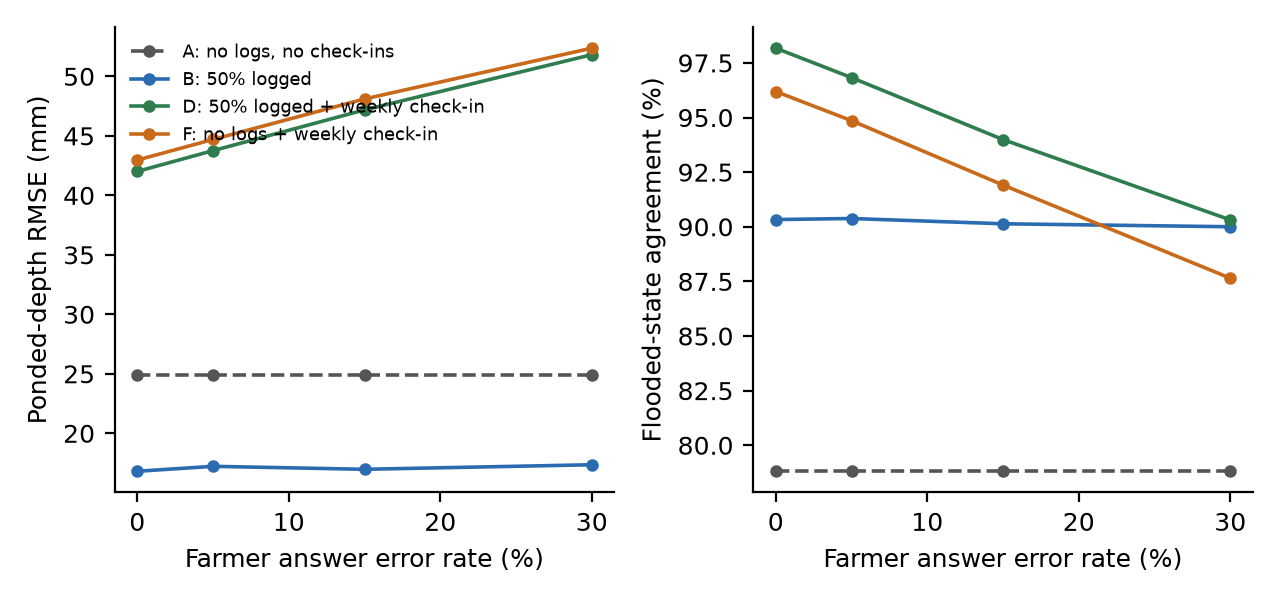
\includegraphics[width=0.78\textwidth]{fig/correction.png}
\caption{Effect of farmer answer error on the rice correction loop. Left: ponded-depth RMSE. Right: agreement of the twin's flooded/dry state with the truth. Condition A (no information) is the flat dashed reference line in each panel.}
\label{fig:correction}
\end{figure}

This is a simulation study whose farmer error model is our assumption; real answer error rates are unknown and are the first quantity a field trial should measure. It uses a synthetic truth field, not real logged irrigation. But the quantisation mechanism it identifies follows directly from the check-in's three-option design and the fixed-confidence correction operator, independent of how realistic the error model is, and points to a specific, low-risk fix: a finer-grained check-in question, or a correction operator that treats a qualitative answer as a soft bound rather than a hard target.

\subsection{Sentinel-1 retrieval over Gorakhpur}

We exercised the satellite pipeline on a pre-specified $4\times3$ grid of points ($26.4$--$27.0^{\circ}$N, $83.2$--$83.6^{\circ}$E), each a $0.004^{\circ}$ square (about 0.4\,km on a side), using six-day Sentinel-1 windows from 1 June to 15 September 2025 (18 windows). Every request went through the statistics client and detection code the application uses. Retrieval is slow, about ten minutes per point, and the run stalled on the Copernicus quota; only the first two grid points were completed, and both are reported in full -- no point was dropped after inspecting results, and the other ten were simply never retrieved.

Sentinel-1 returned a usable observation in 18 of 18 and 17 of 18 windows through the whole monsoon (Table~\ref{tab:sentinel}, Figure~\ref{fig:ponding_sat} right). The two points behave differently. At the first, VH backscatter stays between $-27.2$ and $-15.9$\,dB, with 11 windows below the $-22$\,dB open-water threshold, including a sustained period from early August; the detector reports a transplant signature dated 2025-08-10, with an 11.3\,dB drop and a 5.1\,dB recovery, confidence 1.00. At the second, backscatter rises after mid-June and reaches about $-15$ to $-14$\,dB by August, with only three windows below $-22$\,dB, all in June, and no transplant is detected. We cannot say whether either result is correct, since no ground truth on land cover or transplant date was available at either location; the first trace is compatible with a late-transplanted paddy but equally with inundated low-lying land that was never planted. This exposes a design weakness shared with many flooding detectors built the same way: the detector selects the global minimum of the series, so any persistently flooded surface can produce a signature, and the subsequent check for a rise to canopy-level backscatter is only a partial safeguard. At both points the June windows already show low backscatter, so the observation window should begin earlier than 1 June to capture land preparation and avoid mistaking it for the main transplant event.

\begin{table}[htbp]
\centering
\caption{Sentinel-1 retrieval at the two completed grid points. VH statistics are field-mean values in dB over six-day windows (1 Jun--15 Sep 2025).}
\label{tab:sentinel}
\resizebox{\textwidth}{!}{%
\begin{tabular}{lcccl}
\toprule
Point ($^{\circ}$N, $^{\circ}$E) & Windows w/ data & VH min/med./max (dB) & Windows $<-22$dB & Transplant detected \\
\midrule
26.4, 83.2 & 18/18 & $-27.2$ / $-23.7$ / $-15.9$ & 11 & Yes (2025-08-10, conf.\ 1.00) \\
26.4, 83.4 & 17/18 & $-24.1$ / $-15.4$ / $-13.9$ & 3 & No \\
\bottomrule
\end{tabular}}
\end{table}

\begin{figure}[htbp]
\centering
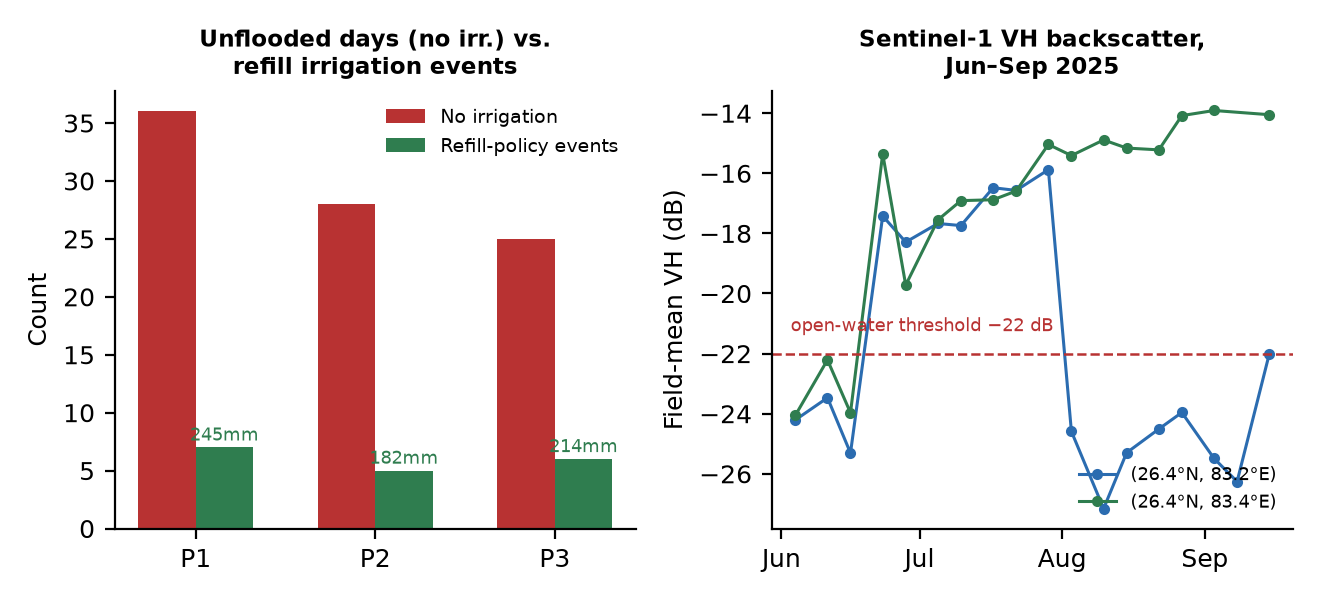
\includegraphics[width=0.92\textwidth]{fig/ponding_sat.png}
\caption{Left: the ponding-management consistency check of Table~\ref{tab:ponding} (unflooded days without irrigation, against the refill policy's irrigation events, with net applied water labelled). Right: Sentinel-1 VH backscatter at the two completed grid points, with the open-water threshold used by the transplant detector.}
\label{fig:ponding_sat}
\end{figure}

\subsection{Disease classifier evaluation}

\subsubsection{In-distribution validation versus cross-dataset generalisation}

The shipped classifier is an EfficientNet-B0 (Tan and Le, 2019) fine-tuned on ten rice leaf-disease classes, trained on a corpus built by merging several public rice-leaf datasets, mapping their folder-level labels onto a single class vocabulary, and removing near-duplicate images with a perceptual hash so that near-identical shots of the same leaf -- common across these datasets -- cannot leak between splits and inflate accuracy. Strong augmentation (random crop, flips, rotation, colour jitter, blur, erasing) and class-balanced sampling were used during training. Critically, the evaluation design keeps two numbers conceptually separate and never averages them together: an \emph{in-distribution validation} split, a random 10\% held out from the same datasets used for training, which measures how well the model fits images like the ones it trained on; and a \emph{held-out test} set consisting of every image from one entire source dataset withheld from training altogether, which measures whether the model has learned the disease or the photographic habits of a particular dataset -- the camera, the background, the lighting, the image-processing pipeline. The two differ sharply (Table~\ref{tab:classifier}, Figure~\ref{fig:disease_eval}).

\begin{table}[htbp]
\centering
\caption{Disease classifier (EfficientNet-B0, 10 classes) evaluation, from the training run's own metrics file.}
\label{tab:classifier}
\begin{tabular}{lcc}
\toprule
Metric & In-distribution validation & Held-out (cross-dataset) \\
\midrule
$n$ & 1496 & 1106 \\
Accuracy & 92.8\% & 20.1\% \\
Macro F1 & 0.940 & 0.162 \\
Expected calibration error (ECE) & 0.067 & 0.513 \\
Withheld by confidence gate ($<0.65$) & 7.2\% & 36.1\% \\
Accuracy among predictions above the gate & 96.0\% & 20.4\% \\
\bottomrule
\end{tabular}
\end{table}

In-distribution, the model is both accurate and well calibrated: 92.8\% accuracy, macro F1 0.940, and an expected calibration error of 0.067 (a model's stated confidence and its actual accuracy track each other closely). On the held-out dataset -- which contained only five of the ten classes, so this number describes generalisation on those five, not all ten -- accuracy collapses to 20.1\% and the calibration error rises to 0.513, meaning the model is now not just wrong but confidently wrong. The clearest illustration is the confidence gate itself: in-distribution, predictions that clear the 0.65 gate are right 96.0\% of the time, exactly what a gate is for. On the held-out set, predictions that clear the \emph{same} gate are right only 20.4\% of the time -- barely different from the held-out set's 20.1\% unfiltered accuracy. The gate, which is genuinely protective in-distribution, provides essentially no protection at all under this kind of distribution shift, precisely because the calibration that makes a gate meaningful has itself broken down. Per-class results sharpen this further: two of the five classes present in the held-out set, which scored a perfect or near-perfect F1 in-distribution (sheath blight 0.963, leaf scald 1.000), fell to a recall of 3\% and under 1\% respectively on the held-out images, despite their in-distribution performance giving no warning of this. Tungro (0.51 recall) and leaf blast (0.41 recall) degraded far less severely, suggesting these two diseases' visual symptoms generalise across photographic sources better than the others do, though still far from reliably.

\begin{figure}[htbp]
\centering
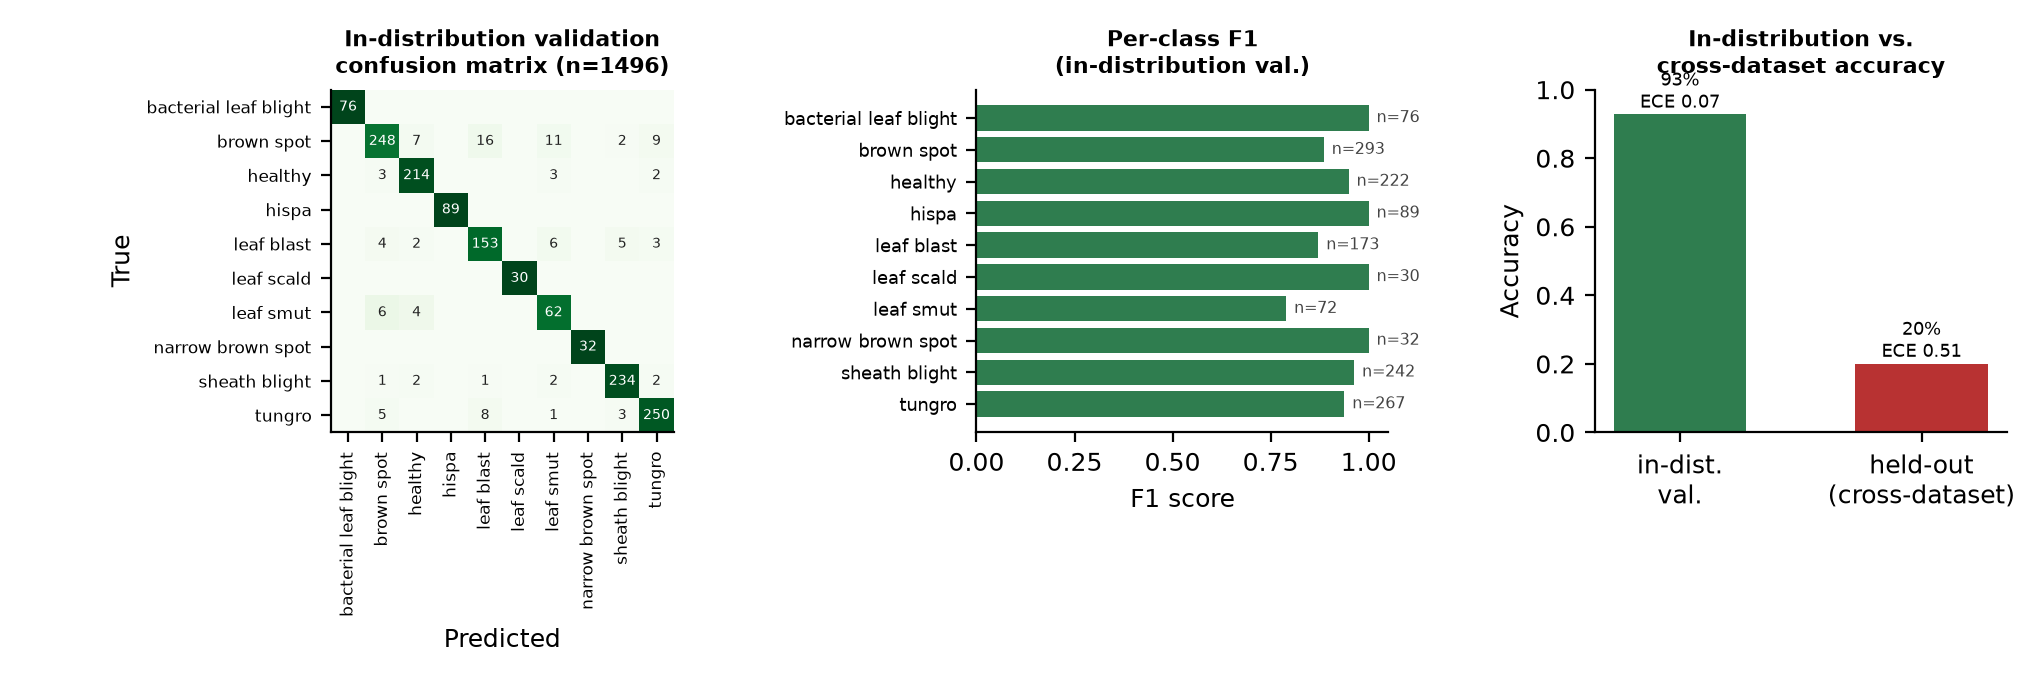
\includegraphics[width=0.98\textwidth]{fig/disease_eval.png}
\caption{Left: in-distribution validation confusion matrix. Middle: per-class F1 in-distribution. Right: in-distribution versus held-out (cross-dataset) accuracy, with expected calibration error (ECE) for each.}
\label{fig:disease_eval}
\end{figure}

\subsubsection{Confidence gating against non-leaf inputs}

A separate failure mode from cross-dataset generalisation is a closed-set classifier's inability to say ``this is not a rice leaf at all''. We stress-tested the shipped weights with 100 images that are not leaves: 20 solid colours, 20 Gaussian-noise images, 20 smooth gradients, 20 stripe patterns and 20 blurred green textures, and compared against the same test run on the earlier four-class ResNet-18 model (Figure~\ref{fig:ood}). The result is a substantial, though incomplete, improvement: the ten-class model accepts only 18\% of these non-leaf images at the deployed 0.65 gate (mean confidence 0.37) against 91\% for the four-class model at the same threshold. The improvement is not uniform across input families -- solid colours (35\%) and stripe patterns (45\%) are still accepted at a troubling rate, while Gaussian noise, gradients and green textures are now almost entirely rejected. We did not design this experiment to isolate why the newer model is harder to fool -- more classes (including the ``healthy'' class acting as a partial catch-all), stronger augmentation, and the larger, more diverse training corpus are all plausible contributors, and distinguishing them would need a controlled ablation we have not run. What the result does establish is that this particular failure mode, unlike cross-dataset generalisation, is one where model and training changes already made measurable, substantial progress, which is encouraging but should not be read as the gate now being adequate: a closed-set softmax still has no genuine ``none of the above'' output, and 18\% of garbage images reaching a farmer with a confident disease name is still a real failure rate.

\begin{figure}[htbp]
\centering
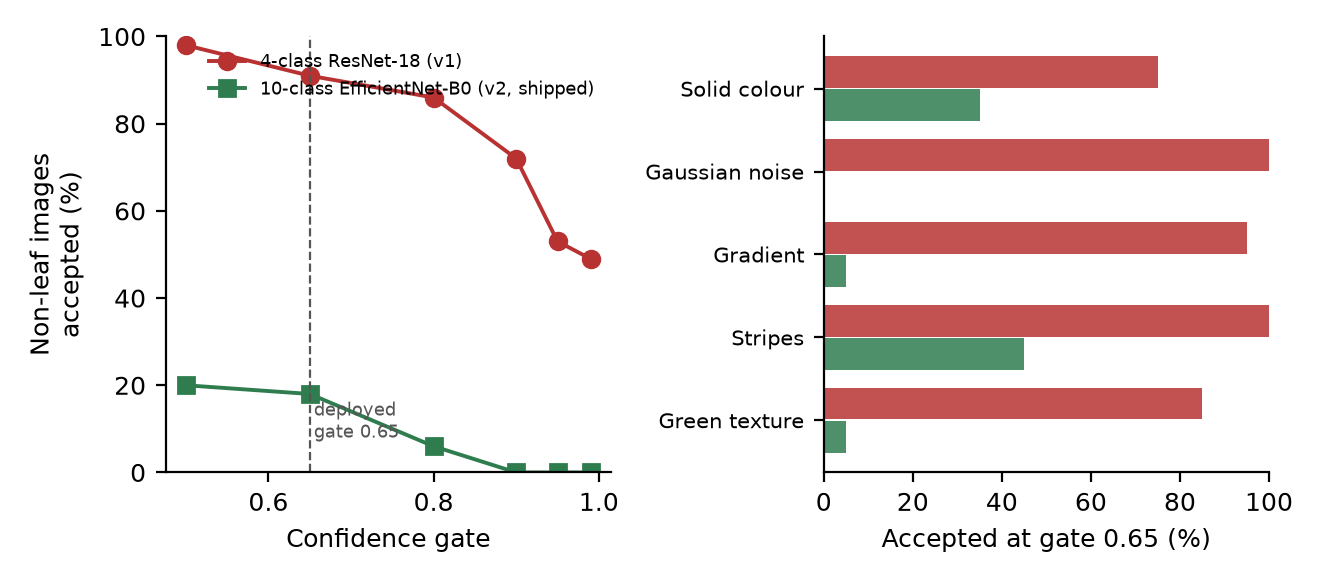
\includegraphics[width=0.92\textwidth]{fig/ood.png}
\caption{Out-of-distribution stress test (100 non-leaf images), four-class ResNet-18 (v1) versus the shipped ten-class EfficientNet-B0 (v2). Left: share of inputs accepted as the confidence gate is raised. Right: share accepted at the deployed gate 0.65, by input family.}
\label{fig:ood}
\end{figure}

\subsubsection{Case study: five field photographs}

As a qualitative, non-statistical check, we ran the shipped classifier with Grad-CAM++ on five real rice-leaf photographs supplied for this paper, none of which are part of the training or evaluation corpus (Figure~\ref{fig:case}). With $n=5$ this is an illustration, not an accuracy estimate. Three predictions cleared the confidence gate: sheath blight at 93\% confidence, with the heatmap concentrated tightly on the visible lesion; brown spot at 77\%, correctly localised on the characteristic oval spots; and healthy at 89\%, where the heatmap is diffuse across the whole leaf blade rather than anchored to any single region -- expected, since there is no lesion for a correct ``healthy'' prediction to point to, and a useful sanity check in itself (a sharply localised heatmap on a ``healthy'' call would be a warning sign of a shortcut). Two predictions fell below the 0.65 gate and were correctly withheld: a leaf-blast call at 60\% confidence (margin to the second class 0.42, still localised reasonably on a lesion) and a bacterial-leaf-blight call at only 33\% confidence (margin 0.15, the heatmap partially on the discoloured leaf collar but partially on an adjacent, healthy-looking stem) -- exactly the kind of ambiguous image the gate exists to catch, and in this small sample, it did.

\begin{figure}[htbp]
\centering
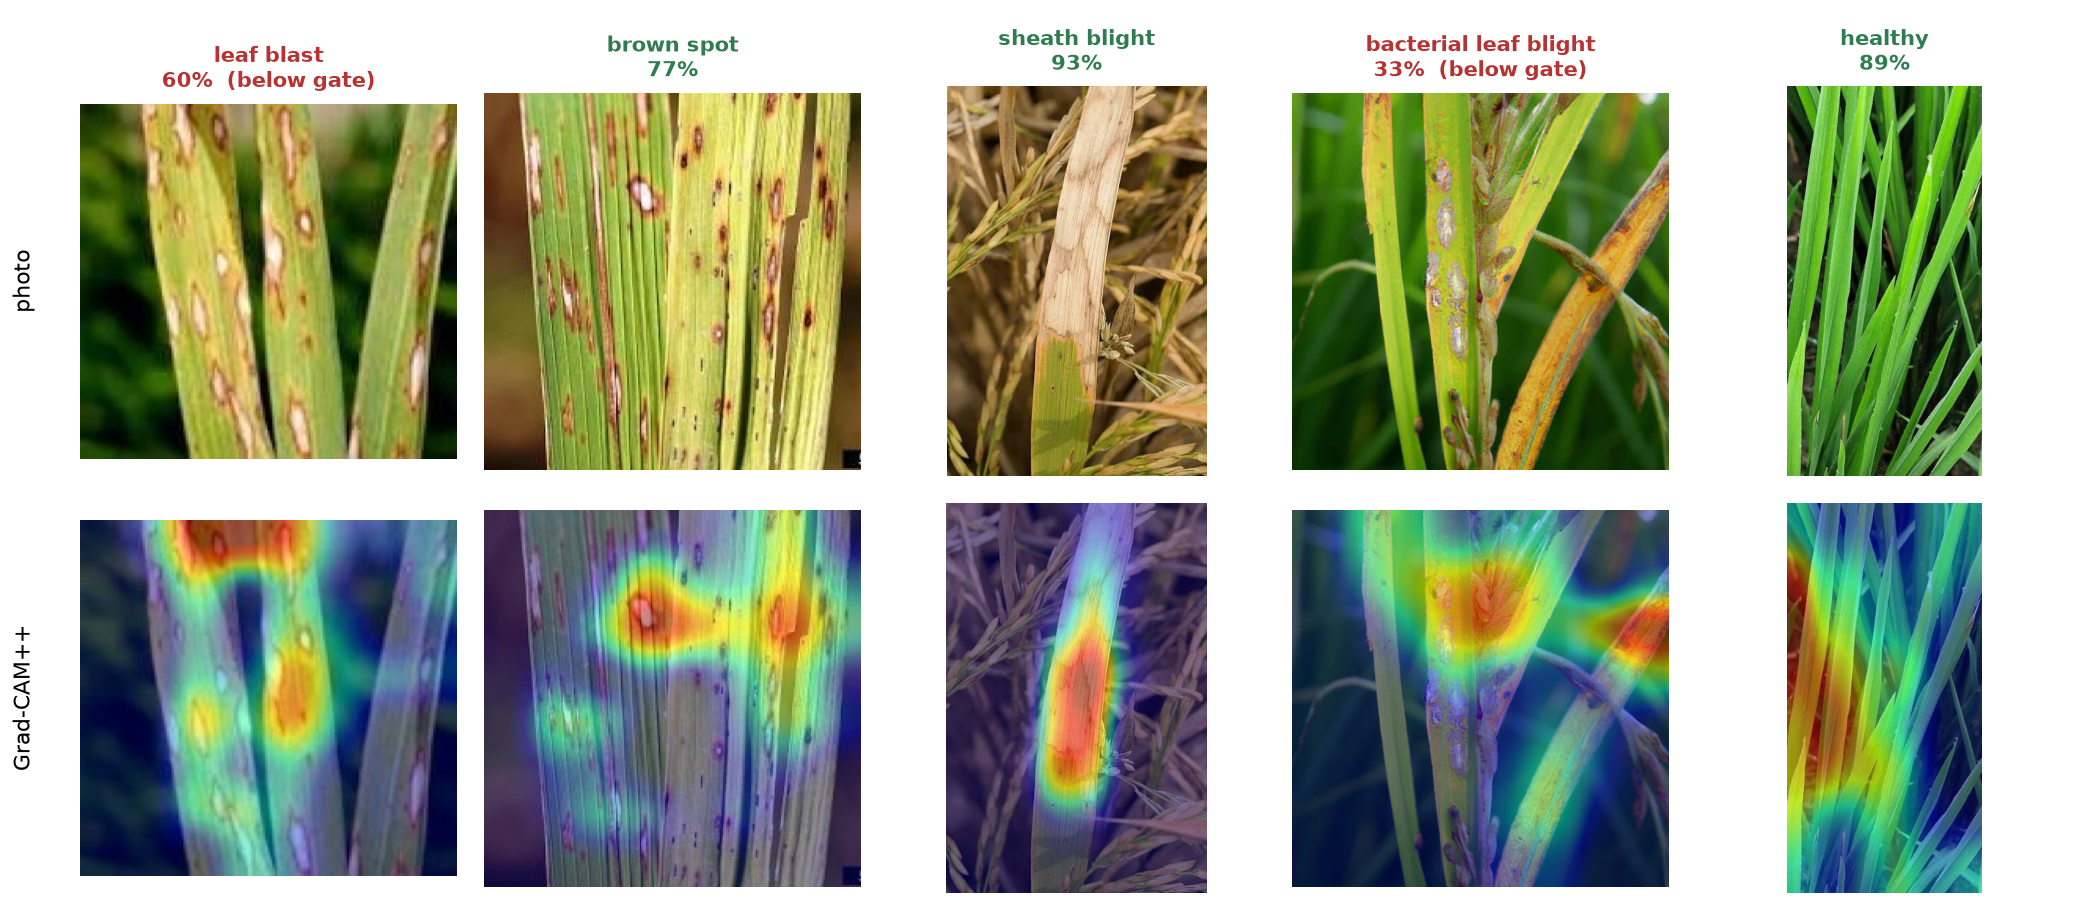
\includegraphics[width=0.98\textwidth]{fig/case_study.png}
\caption{Five real field photographs, classifier prediction and confidence, and the Grad-CAM++ attention overlay. The two below-gate predictions (red) are correctly withheld by the confidence gate rather than shown to the farmer as treatment advice.}
\label{fig:case}
\end{figure}

\section{Discussion}

\textbf{What the evidence supports.} The physical core is numerically consistent with the FAO-56 references, closes its water balance to rounding error, and follows an independent ET\textsubscript{0} product over a full rice season (Sections 4.2--4.3). The ponded-depth model is a genuine correction of an earlier design error, not merely a relabelling, and the season's rainfall happened to protect the flowering window at all three simulated points even without irrigation (Section 4.4). The satellite pipeline retrieves real, physically sensible data through the free Copernicus service (Section 4.7), and every farmer-facing output reads one shared state.

\textbf{What it does not support.} We cannot claim the twin predicts transplant dates or flooding status correctly, because no ground truth was measured; the Sentinel-1 detector's reliance on a global backscatter minimum is a known weakness, not just an unverified result. We cannot claim disease-diagnosis accuracy in the field: Section 4.8's own training-run metrics show a 73-percentage-point gap between validation-split and cross-dataset accuracy, and that gap, measured on the model's own evaluation protocol rather than inferred indirectly, is a stronger and more specific finding than the earlier out-of-distribution stress test alone would have supported.

\textbf{Findings that change the design.} Three results are actionable. (i) The farmer-correction simulation shows check-ins improve the operationally relevant flooded/dry classification but not the continuous ponded-depth estimate, because the check-in's three discrete answer options quantise a continuous state; a finer-grained question or a soft-bound correction (rather than a blend toward a fixed target) should fix this without weakening the flooded/dry signal (Section 4.6). (ii) The refill irrigation policy, reacting only to the current pond level, loses water to bund overflow disproportionately at the wettest of the three simulated points; a forecast-aware refill rule is a direct improvement available from data the twin already ingests (Section 4.5). (iii) The disease classifier's headline validation accuracy (92.8\%) is not a safe number to show a farmer or cite as the system's accuracy: the held-out cross-dataset result (20.1\%) is the honest estimate of unfamiliar-camera, unfamiliar-background performance, and the confidence gate -- effective in-distribution -- does not recover this gap, because the model's confidence itself is miscalibrated off-distribution. Before this pathway is relied on beyond decision support, it needs either training data broadened to match the diversity of real farmer photography, an explicit distribution-shift detector separate from the classification confidence, or both; the non-leaf confidence gate, while substantially improved over the earlier four-class model, is a different and narrower safeguard that does not address this gap.

\textbf{Threats to validity.} The ET\textsubscript{0} intercomparison uses a related model product, not a ground station. The ponding and correction studies assume a specific refill policy and a specific synthetic farmer error model; real irrigation behaviour and real answer error rates are unmeasured. The Sentinel-1 results cover two points without ground truth. Three points in one district and one season limit generality, and the region constants are literature defaults pending a season of local ground truth. The classifier's held-out evaluation, while methodologically the most informative experiment in this paper, still reflects only one external dataset's photographic style against the training corpus's; a different external source could show a smaller or larger gap, and the five-image case study is illustrative, not statistical.

\section{Conclusion and Future Work}

FarmSense shows that a compact FAO-56-based crop twin, parameterised by region and assimilating satellite, farmer and photographic observations, can be built from open data and run per field per day for ponded rice, with a water model that correctly represents paddy as a standing-water system rather than a relabelled upland soil bucket. Critical evaluation exposed three weaknesses that a demonstration would have hidden: a check-in design that improves categorical agreement while not improving (and sometimes worsening) the underlying continuous estimate, an irrigation policy that is wasteful under abundant rainfall, and -- most importantly -- a disease classifier whose own training-run evaluation shows a severe, specific, and previously unquantified cross-dataset generalisation gap that a confidence gate alone does not close. The next steps are (a) broadening the disease-classifier training corpus with photographs matching real farmer camera conditions, and evaluating any future retrain with the same in-distribution/held-out split discipline used here, since it is what surfaced the gap in the first place; (b) a season-long field trial that measures real irrigation logging rates, farmer answer error, and actual transplant and flooding dates, to calibrate the correction weights and validate the Sentinel-1 detector against ground truth; (c) a finer-grained or soft-bound check-in correction for ponded depth; and (d) a forecast-aware refill policy and offline operation for the intended field-connectivity conditions.

\section*{Data and Code Availability}

The experiment scripts are in the project's \texttt{backend/experiments} directory, with the raw result files they produced in \texttt{backend/experiments/results}; the figures in this paper are generated from those files by \texttt{backend/experiments/paper\_figs.py} with no numbers transcribed by hand. The disease-classifier metrics are read directly from \texttt{ai/models/rice\_v2/metrics.json}, written by the training run and, per the project's own stated convention, the only place an accuracy number for this component should be quoted from. They read only public data (Open-Meteo, NASA POWER, ISRIC SoilGrids, Copernicus Data Space) and the project source code, and random processes are seeded. The Copernicus retrievals need a free CDSE account.

\section*{References}
\refitem{Allen, R.G., Pereira, L.S., Raes, D. and Smith, M. (1998) \textit{Crop evapotranspiration: guidelines for computing crop water requirements}. FAO Irrigation and Drainage Paper 56. Rome: Food and Agriculture Organization of the United Nations.}
\refitem{Bazzi, H., Baghdadi, N., El Hajj, M., Zribi, M., Minh, D.H.T., Ndikumana, E., Courault, D. and Belhouchette, H. (2019) `Mapping paddy rice using Sentinel-1 SAR time series in Camargue, France', \textit{Remote Sensing}, 11(7), article 887.}
\refitem{Bouman, B.A.M., Lampayan, R.M. and Tuong, T.P. (2007) \textit{Water management in irrigated rice: coping with water scarcity}. Los Baños: International Rice Research Institute.}
\refitem{Chattopadhay, A., Sarkar, A., Howlader, P. and Balasubramanian, V.N. (2018) `Grad-CAM++: generalized gradient-based visual explanations for deep convolutional networks', in \textit{2018 IEEE Winter Conference on Applications of Computer Vision (WACV)}, pp.\ 839--847.}
\refitem{Evensen, G. (2003) `The ensemble Kalman filter: theoretical formulation and practical implementation', \textit{Ocean Dynamics}, 53(4), pp.\ 343--367.}
\refitem{Ferentinos, K.P. (2018) `Deep learning models for plant disease detection and diagnosis', \textit{Computers and Electronics in Agriculture}, 145, pp.\ 311--318.}
\refitem{Grieves, M. and Vickers, J. (2017) `Digital twin: mitigating unpredictable, undesirable emergent behavior in complex systems', in Kahlen, F.-J., Flumerfelt, S. and Alves, A. (eds.) \textit{Transdisciplinary perspectives on complex systems}. Cham: Springer, pp.\ 85--113.}
\refitem{Guo, C., Pleiss, G., Sun, Y. and Weinberger, K.Q. (2017) `On calibration of modern neural networks', in \textit{Proceedings of the 34th International Conference on Machine Learning}, PMLR 70, pp.\ 1321--1330.}
\refitem{He, K., Zhang, X., Ren, S. and Sun, J. (2016) `Deep residual learning for image recognition', in \textit{Proceedings of the IEEE Conference on Computer Vision and Pattern Recognition}, pp.\ 770--778.}
\refitem{Hendrycks, D. and Gimpel, K. (2017) `A baseline for detecting misclassified and out-of-distribution examples in neural networks', in \textit{Proceedings of the 5th International Conference on Learning Representations}.}
\refitem{Hengl, T., Mendes de Jesus, J., Heuvelink, G.B.M., Ruiperez Gonzalez, M., Kilibarda, M., Blagoti\'{c}, A. et al. (2017) `SoilGrids250m: global gridded soil information based on machine learning', \textit{PLoS ONE}, 12(2), article e0169748.}
\refitem{Ji, Z., Lee, N., Frieske, R., Yu, T., Su, D., Xu, Y., Ishii, E., Bang, Y.J., Madotto, A. and Fung, P. (2023) `Survey of hallucination in natural language generation', \textit{ACM Computing Surveys}, 55(12), article 248.}
\refitem{Jones, J.W., Hoogenboom, G., Porter, C.H., Boote, K.J., Batchelor, W.D., Hunt, L.A., Wilkens, P.W., Singh, U., Gijsman, A.J. and Ritchie, J.T. (2003) `The DSSAT cropping system model', \textit{European Journal of Agronomy}, 18(3--4), pp.\ 235--265.}
\refitem{Kamilaris, A. and Prenafeta-Boldú, F.X. (2018) `Deep learning in agriculture: a survey', \textit{Computers and Electronics in Agriculture}, 147, pp.\ 70--90.}
\refitem{Keating, B.A., Carberry, P.S., Hammer, G.L., Probert, M.E., Robertson, M.J., Holzworth, D. et al. (2003) `An overview of APSIM, a model designed for farming systems simulation', \textit{European Journal of Agronomy}, 18(3--4), pp.\ 267--288.}
\refitem{Lewis, P., Perez, E., Piktus, A., Petroni, F., Karpukhin, V., Goyal, N. et al. (2020) `Retrieval-augmented generation for knowledge-intensive NLP tasks', in \textit{Advances in Neural Information Processing Systems 33}, pp.\ 9459--9474.}
\refitem{Mohanty, S.P., Hughes, D.P. and Salathé, M. (2016) `Using deep learning for image-based plant disease detection', \textit{Frontiers in Plant Science}, 7, article 1419.}
\refitem{Poggio, L., de Sousa, L.M., Batjes, N.H., Heuvelink, G.B.M., Kempen, B., Ribeiro, E. and Rossiter, D. (2021) `SoilGrids 2.0: producing soil information for the globe with quantified spatial uncertainty', \textit{SOIL}, 7(1), pp.\ 217--240.}
\refitem{Raes, D., Steduto, P., Hsiao, T.C. and Fereres, E. (2009) `AquaCrop---the FAO crop model to simulate yield response to water: II. Main algorithms and software description', \textit{Agronomy Journal}, 101(3), pp.\ 438--447.}
\refitem{Ramcharan, A., McCloskey, P., Baranowski, K., Mbilinyi, N., Mrisho, L., Ndalahwa, M., Legg, J. and Hughes, D.P. (2019) `A mobile-based deep learning model for cassava disease diagnosis', \textit{Frontiers in Plant Science}, 10, article 272.}
\refitem{Selvaraju, R.R., Cogswell, M., Das, A., Vedantam, R., Parikh, D. and Batra, D. (2017) `Grad-CAM: visual explanations from deep networks via gradient-based localization', in \textit{Proceedings of the IEEE International Conference on Computer Vision}, pp.\ 618--626.}
\refitem{Sparks, A.H. (2018) `nasapower: a NASA POWER global meteorology, surface solar energy and climatology data client for R', \textit{Journal of Open Source Software}, 3(30), article 1035.}
\refitem{Tan, M. and Le, Q. (2019) `EfficientNet: rethinking model scaling for convolutional neural networks', in \textit{Proceedings of the 36th International Conference on Machine Learning}, PMLR 97, pp.\ 6105--6114.}
\refitem{Torres, R., Snoeij, P., Geudtner, D., Bibby, D., Davidson, M., Attema, E. et al. (2012) `GMES Sentinel-1 mission', \textit{Remote Sensing of Environment}, 120, pp.\ 9--24.}
\refitem{Verdouw, C., Tekinerdogan, B., Beulens, A. and Wolfert, S. (2021) `Digital twins in smart farming', \textit{Agricultural Systems}, 189, article 103046.}
\refitem{Wolfert, S., Ge, L., Verdouw, C. and Bogaardt, M.-J. (2017) `Big data in smart farming -- a review', \textit{Agricultural Systems}, 153, pp.\ 69--80.}
\refitem{Yao, S., Zhao, J., Yu, D., Du, N., Shafran, I., Narasimhan, K. and Cao, Y. (2023) `ReAct: synergizing reasoning and acting in language models', in \textit{Proceedings of the 11th International Conference on Learning Representations}.}
\refitem{Zippenfenig, P. (2023) \textit{Open-Meteo.com weather API} [Software]. Zenodo. doi:10.5281/zenodo.7970649.}

\end{document}
